%%%%%%%%%%%%%%%%%%%%%%%%%%%%%%%%%%%%%%%%%%%%%%%%%%%%%%%%%%%%
%% Flight Log Wall-Effect Analysis Report
%% 独立コンパイル可能なドキュメント
%% 本文: 日本語  /  図表キャプション: 英語
%%%%%%%%%%%%%%%%%%%%%%%%%%%%%%%%%%%%%%%%%%%%%%%%%%%%%%%%%%%%
\documentclass[11pt,a4paper]{ltjsarticle}

%%% Packages %%%
\usepackage{luatexja-fontspec}
\usepackage{graphicx}
\usepackage{amsmath,amssymb}
\usepackage{booktabs}
\usepackage[margin=22mm]{geometry}
\usepackage{setspace}
\usepackage[hidelinks]{hyperref}
\usepackage{xcolor}
\usepackage{caption}
\usepackage{subcaption}
\usepackage{float}

\onehalfspacing
\graphicspath{{analysis_output/}}

%%% Title %%%
\title{\textbf{フライトログに基づく壁効果の定量解析}\\[4pt]
\large Wall-Effect Characterisation from PX4 Flight Logs}
\author{}
\date{\today}

\begin{document}
\maketitle

%%%%%%%%%%%%%%%%%%%%%%%%%%%%%%%%%%%%%%%%%%%%%%%%%%%%%%%%%%%%
\section{実験概要}\label{sec:overview}
%%%%%%%%%%%%%%%%%%%%%%%%%%%%%%%%%%%%%%%%%%%%%%%%%%%%%%%%%%%%

本ドキュメントは, ベンチ台に固定したドローンを PX4 STABILIZED モードで自動飛行させた際の ULog フライトログを解析し, 壁近接時の空力外乱（壁効果）を定量評価した結果をまとめたものである.

\subsection{飛行シーケンス}

飛行スクリプト \texttt{forward\_and\_stop.py} により, 以下の 4 フェーズを自動実行した:
\begin{enumerate}
    \item \textbf{Hover1}（壁なし）: アーム直後のホバリング安定化（約 4\,s）
    \item \textbf{Forward}: Pitch 指令による前進（壁に接近, 約 3.5\,s）
    \item \textbf{Brake}: 逆 Pitch 指令による制動（約 1\,s）
    \item \textbf{Hover2}（壁近接）: 壁近傍でのホバリング安定化（約 4\,s）
\end{enumerate}

Hover1 と Hover2 の比較により, 同一スロットル・同一姿勢指令下での壁効果の影響を評価する. フェーズ検出は \texttt{manual\_control\_setpoint} トピックの Pitch 指令遷移から自動的に行った.

\subsection{過渡状態の除去}

Hover1 はアーム直後のスピンアップ過渡を, Hover2 は Brake フェーズからの遷移を含む. これらの非定常区間が統計指標を歪めることを防ぐため, 各ホバリングフェーズの先頭 1.5\,s を評価対象から除外した. タイムラインプロットではフェーズ帯を元の範囲で表示するが, ボックスプロット・統計検定・PSD 等のすべての定量評価にはトリミング後のデータのみを使用している.

\subsection{データセット}

合計 15 本のフライトログを取得し, 制御コマンド条件に基づき 2 グループに分類した (Table~\ref{tab:groups}).

\begin{table}[H]
\centering
\caption{Flight log groups and command parameters.}
\label{tab:groups}
\begin{tabular}{lcccc}
\toprule
Group & Runs & Roll cmd & Fwd pitch & Timestamp \\
\midrule
A (baseline?) & 4 & $-0.10 \sim -0.16$ & $-0.06 \sim -0.07$ & 11:20--14:37 \\
B (morphed?)  & 11 & $-0.20$ & $-0.09$ & 15:46--16:05 \\
\bottomrule
\end{tabular}
\end{table}

Roll コマンドの差はトリム補正であり, 機体変形に伴う空力バイアスを打ち消すために意図的に設定したものである. したがって, トリム値の違いは機体構成の違いを反映している.

%%%%%%%%%%%%%%%%%%%%%%%%%%%%%%%%%%%%%%%%%%%%%%%%%%%%%%%%%%%%
\section{単一ラン解析}\label{sec:single_run}
%%%%%%%%%%%%%%%%%%%%%%%%%%%%%%%%%%%%%%%%%%%%%%%%%%%%%%%%%%%%

\subsection{Group B 代表ラン}

Group B の代表ラン（\texttt{log\_34}）について, 全チャネルのタイムラインを Fig.~\ref{fig:timeline_b} に示す. 4 フェーズがカラー帯で表示されている.

\begin{figure}[H]
\centering

\includegraphics[width=\linewidth]{plot1_timeline.png}
\caption{Flight timeline for Group~B representative run (\texttt{log\_34}). Six channels are shown: pitch angle (setpoint vs.\ actual), roll angle, roll rate, motor commands (M0--M3), thrust setpoint, and torque setpoint. Coloured bands indicate the four flight phases.}
\label{fig:timeline_b}
\end{figure}

Fig.~\ref{fig:roll_detail_b} に Hover1 と Hover2 の Roll 外乱を詳細比較する. 先頭 1.5\,s を除去した安定区間のみを対象としている. 左列は位相合わせした時系列のオーバーレイ, 右列はボックスプロットである. Hover2 では Roll rate と Roll torque の振幅が Hover1 より明確に増大している.

\begin{figure}[H]
\centering

\includegraphics[width=\linewidth]{plot2_roll_detail.png}
\caption{Roll disturbance comparison between Hover1 (no wall) and Hover2 (near wall) for Group~B representative run. The initial 1.5\,s transient is excluded. Top: roll angle, middle: roll rate, bottom: roll torque setpoint. Left: phase-aligned time series, right: box plots.}
\label{fig:roll_detail_b}
\end{figure}

Fig.~\ref{fig:motors_b} にモータ出力の解析を示す. M1--M3 非対称度が Hover1 ではほぼゼロだが, Hover2 では正方向にシフトしており, 壁側と非壁側のモータ出力バランスが壁近接で崩れていることがわかる.

\begin{figure}[H]
\centering

\includegraphics[width=\linewidth]{plot3_motors.png}
\caption{Motor output analysis for Group~B representative run. Top: motor command time series. Middle-left: normalised asymmetry (M0--M2 and M1--M3). Middle-right: M1--M3 asymmetry box plot by phase. Bottom-left: radar chart of mean motor balance. Bottom-right: motor output variability (std) by phase.}
\label{fig:motors_b}
\end{figure}

Fig.~\ref{fig:psd_b} に周波数解析結果を示す. Hover2 では低周波域（$<20$\,Hz）で Roll ジャイロの PSD が増大しており, 壁効果が低周波の外乱として作用していることを示唆する.

\begin{figure}[H]
\centering

\includegraphics[width=\linewidth]{plot4_psd.png}
\caption{Power spectral density (PSD) analysis for Group~B representative run. Top-left: roll gyro PSD (Hover1 vs.\ Hover2). Top-right: pitch gyro PSD. Bottom-left: roll gyro PSD for all four phases. Bottom-right: lateral acceleration (Y-axis) PSD.}
\label{fig:psd_b}
\end{figure}

Fig.~\ref{fig:control_effort_b} に制御努力の解析を示す. Hover2 では Roll トルク RMS が Hover1 より増大しており, コントローラが壁効果の補償に追加の制御努力を要していることがわかる.

\begin{figure}[H]
\centering

\includegraphics[width=\linewidth]{plot6_control_effort.png}
\caption{Control effort analysis for Group~B representative run. Top: rate controller integral terms. Middle: rolling-window RMS of torque setpoint (roll and pitch). Bottom: motor power proxy ($\sum \mathrm{cmd}^2$).}
\label{fig:control_effort_b}
\end{figure}

\subsection{Group A 代表ラン}

Group A の代表ラン（\texttt{log\_0}）のタイムラインと Roll 外乱比較を Fig.~\ref{fig:timeline_a}--\ref{fig:roll_detail_a} に示す. Group A では Hover2 における Roll rate の変動が Group B より顕著に大きい.

\begin{figure}[H]
\centering
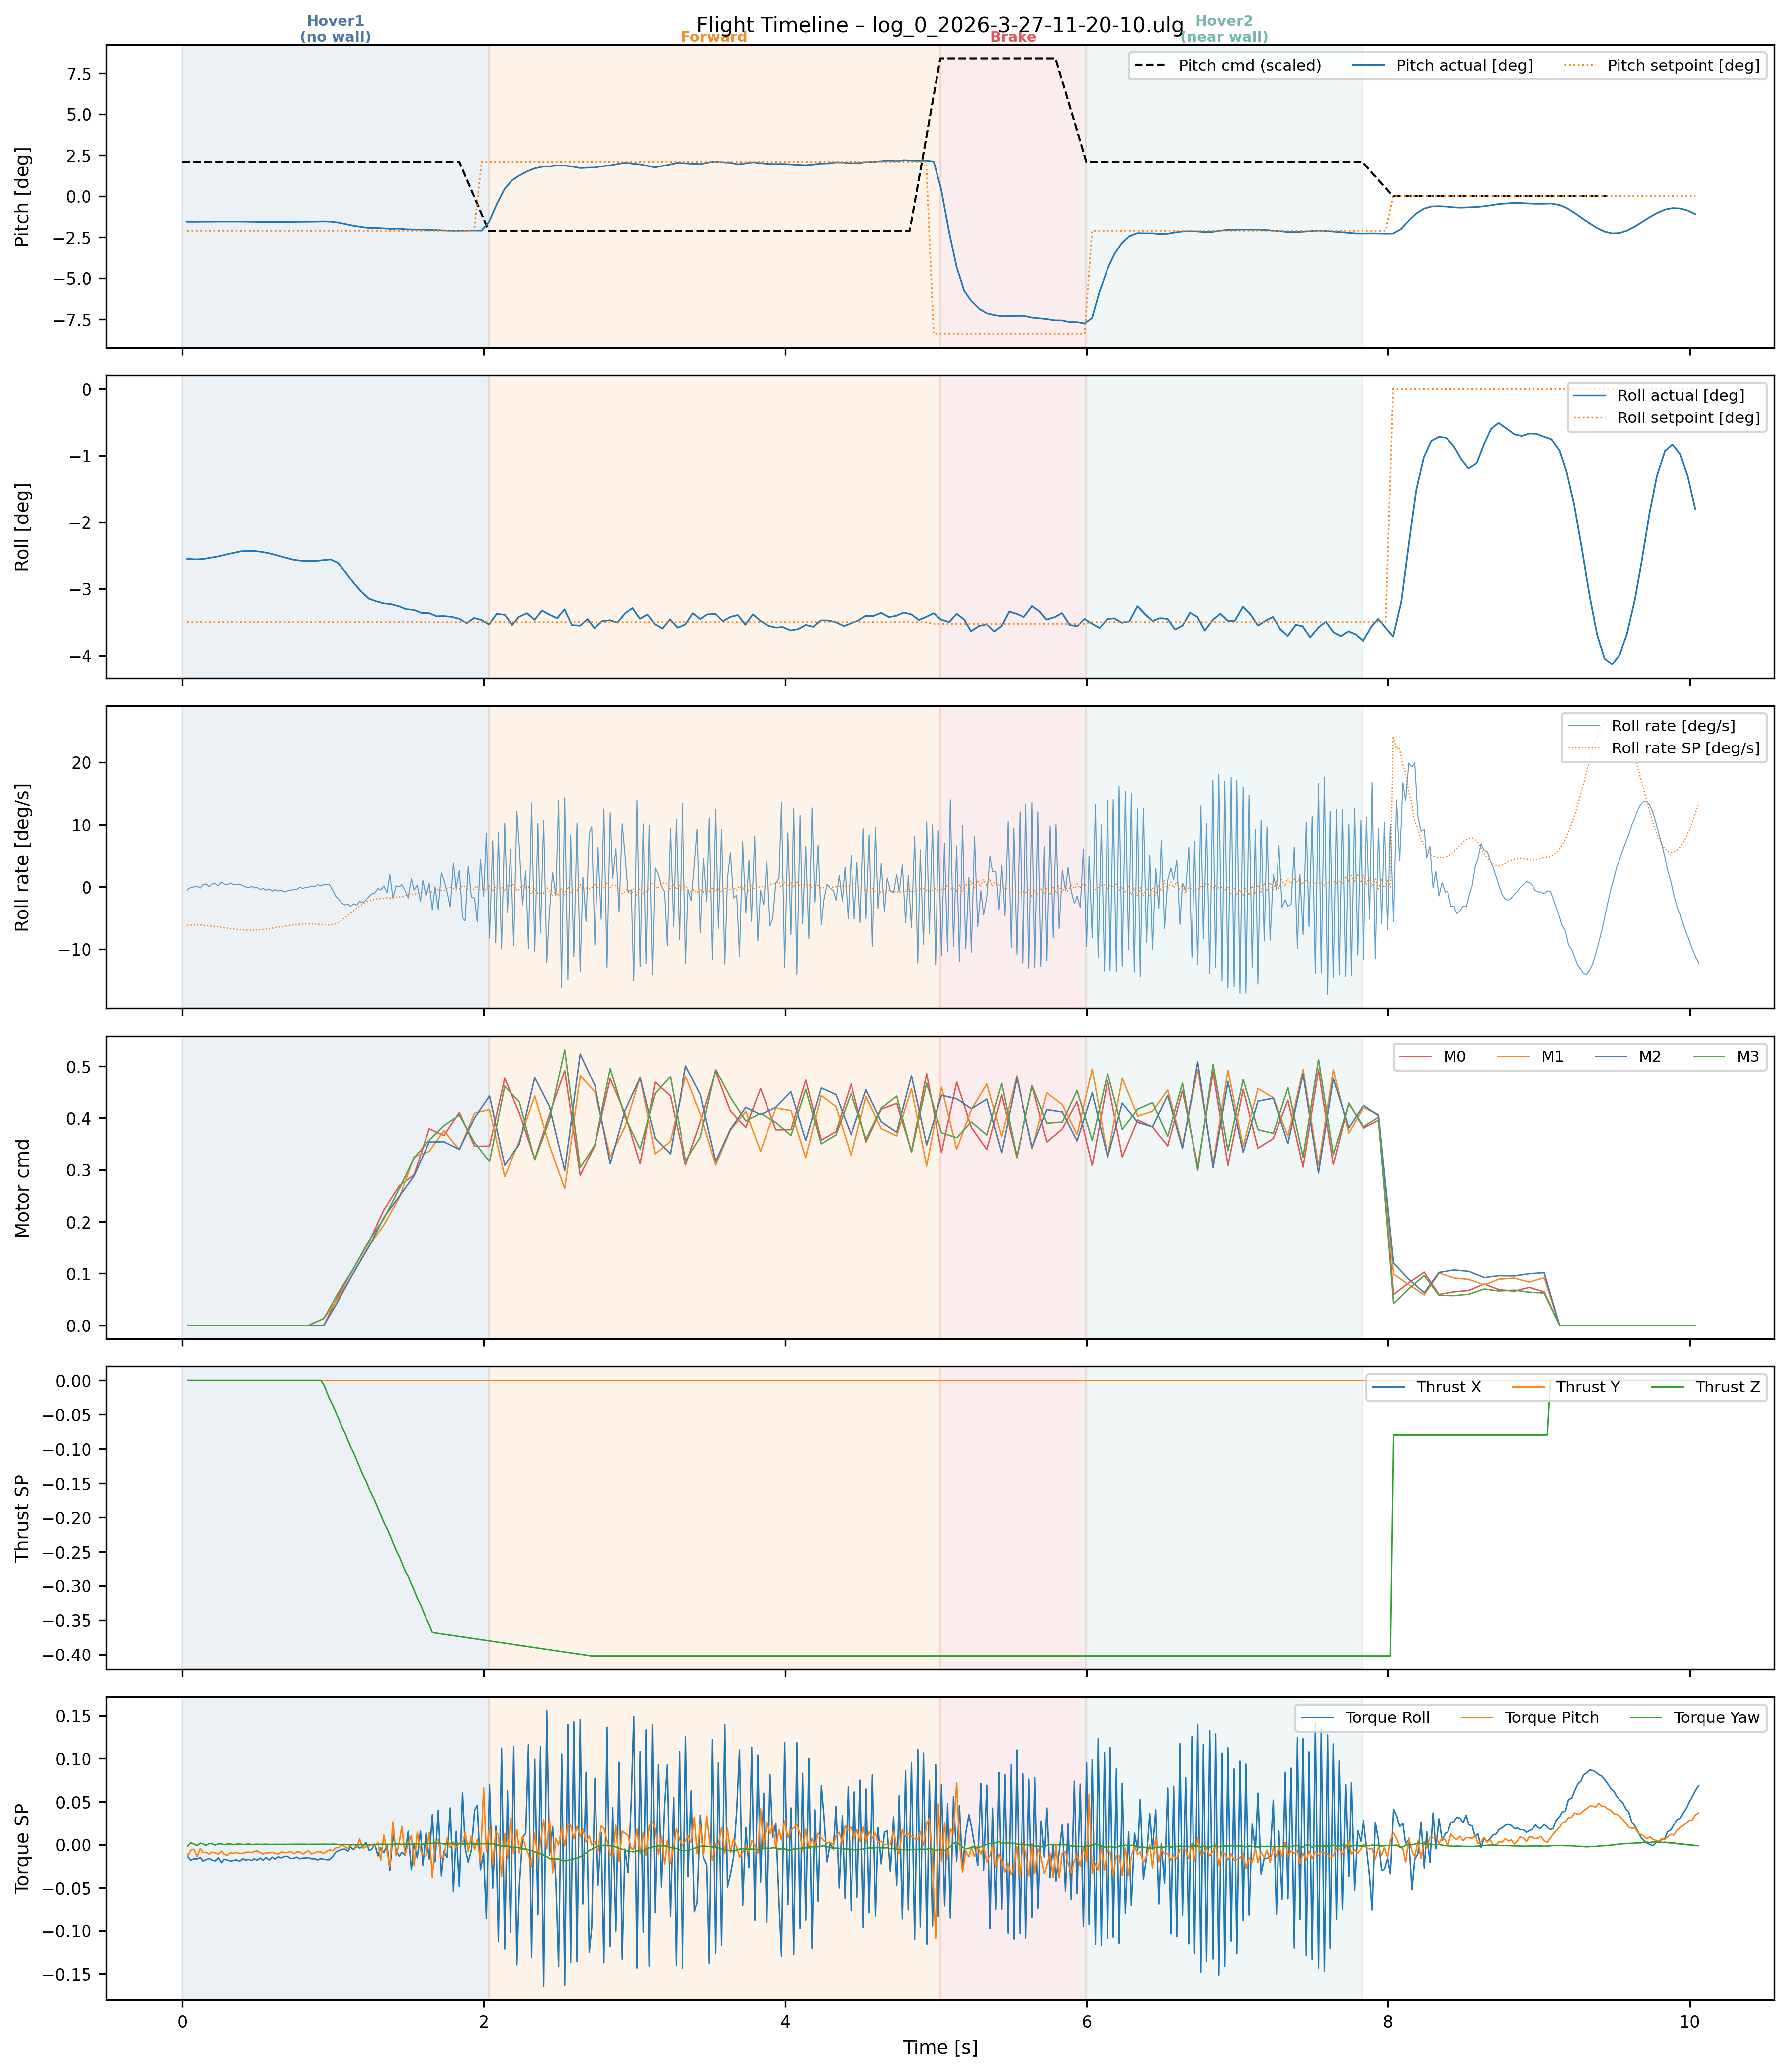
\includegraphics[width=\linewidth]{group_a/plot1_timeline.png}
\caption{Flight timeline for Group~A representative run (\texttt{log\_0}).}
\label{fig:timeline_a}
\end{figure}

\begin{figure}[H]
\centering
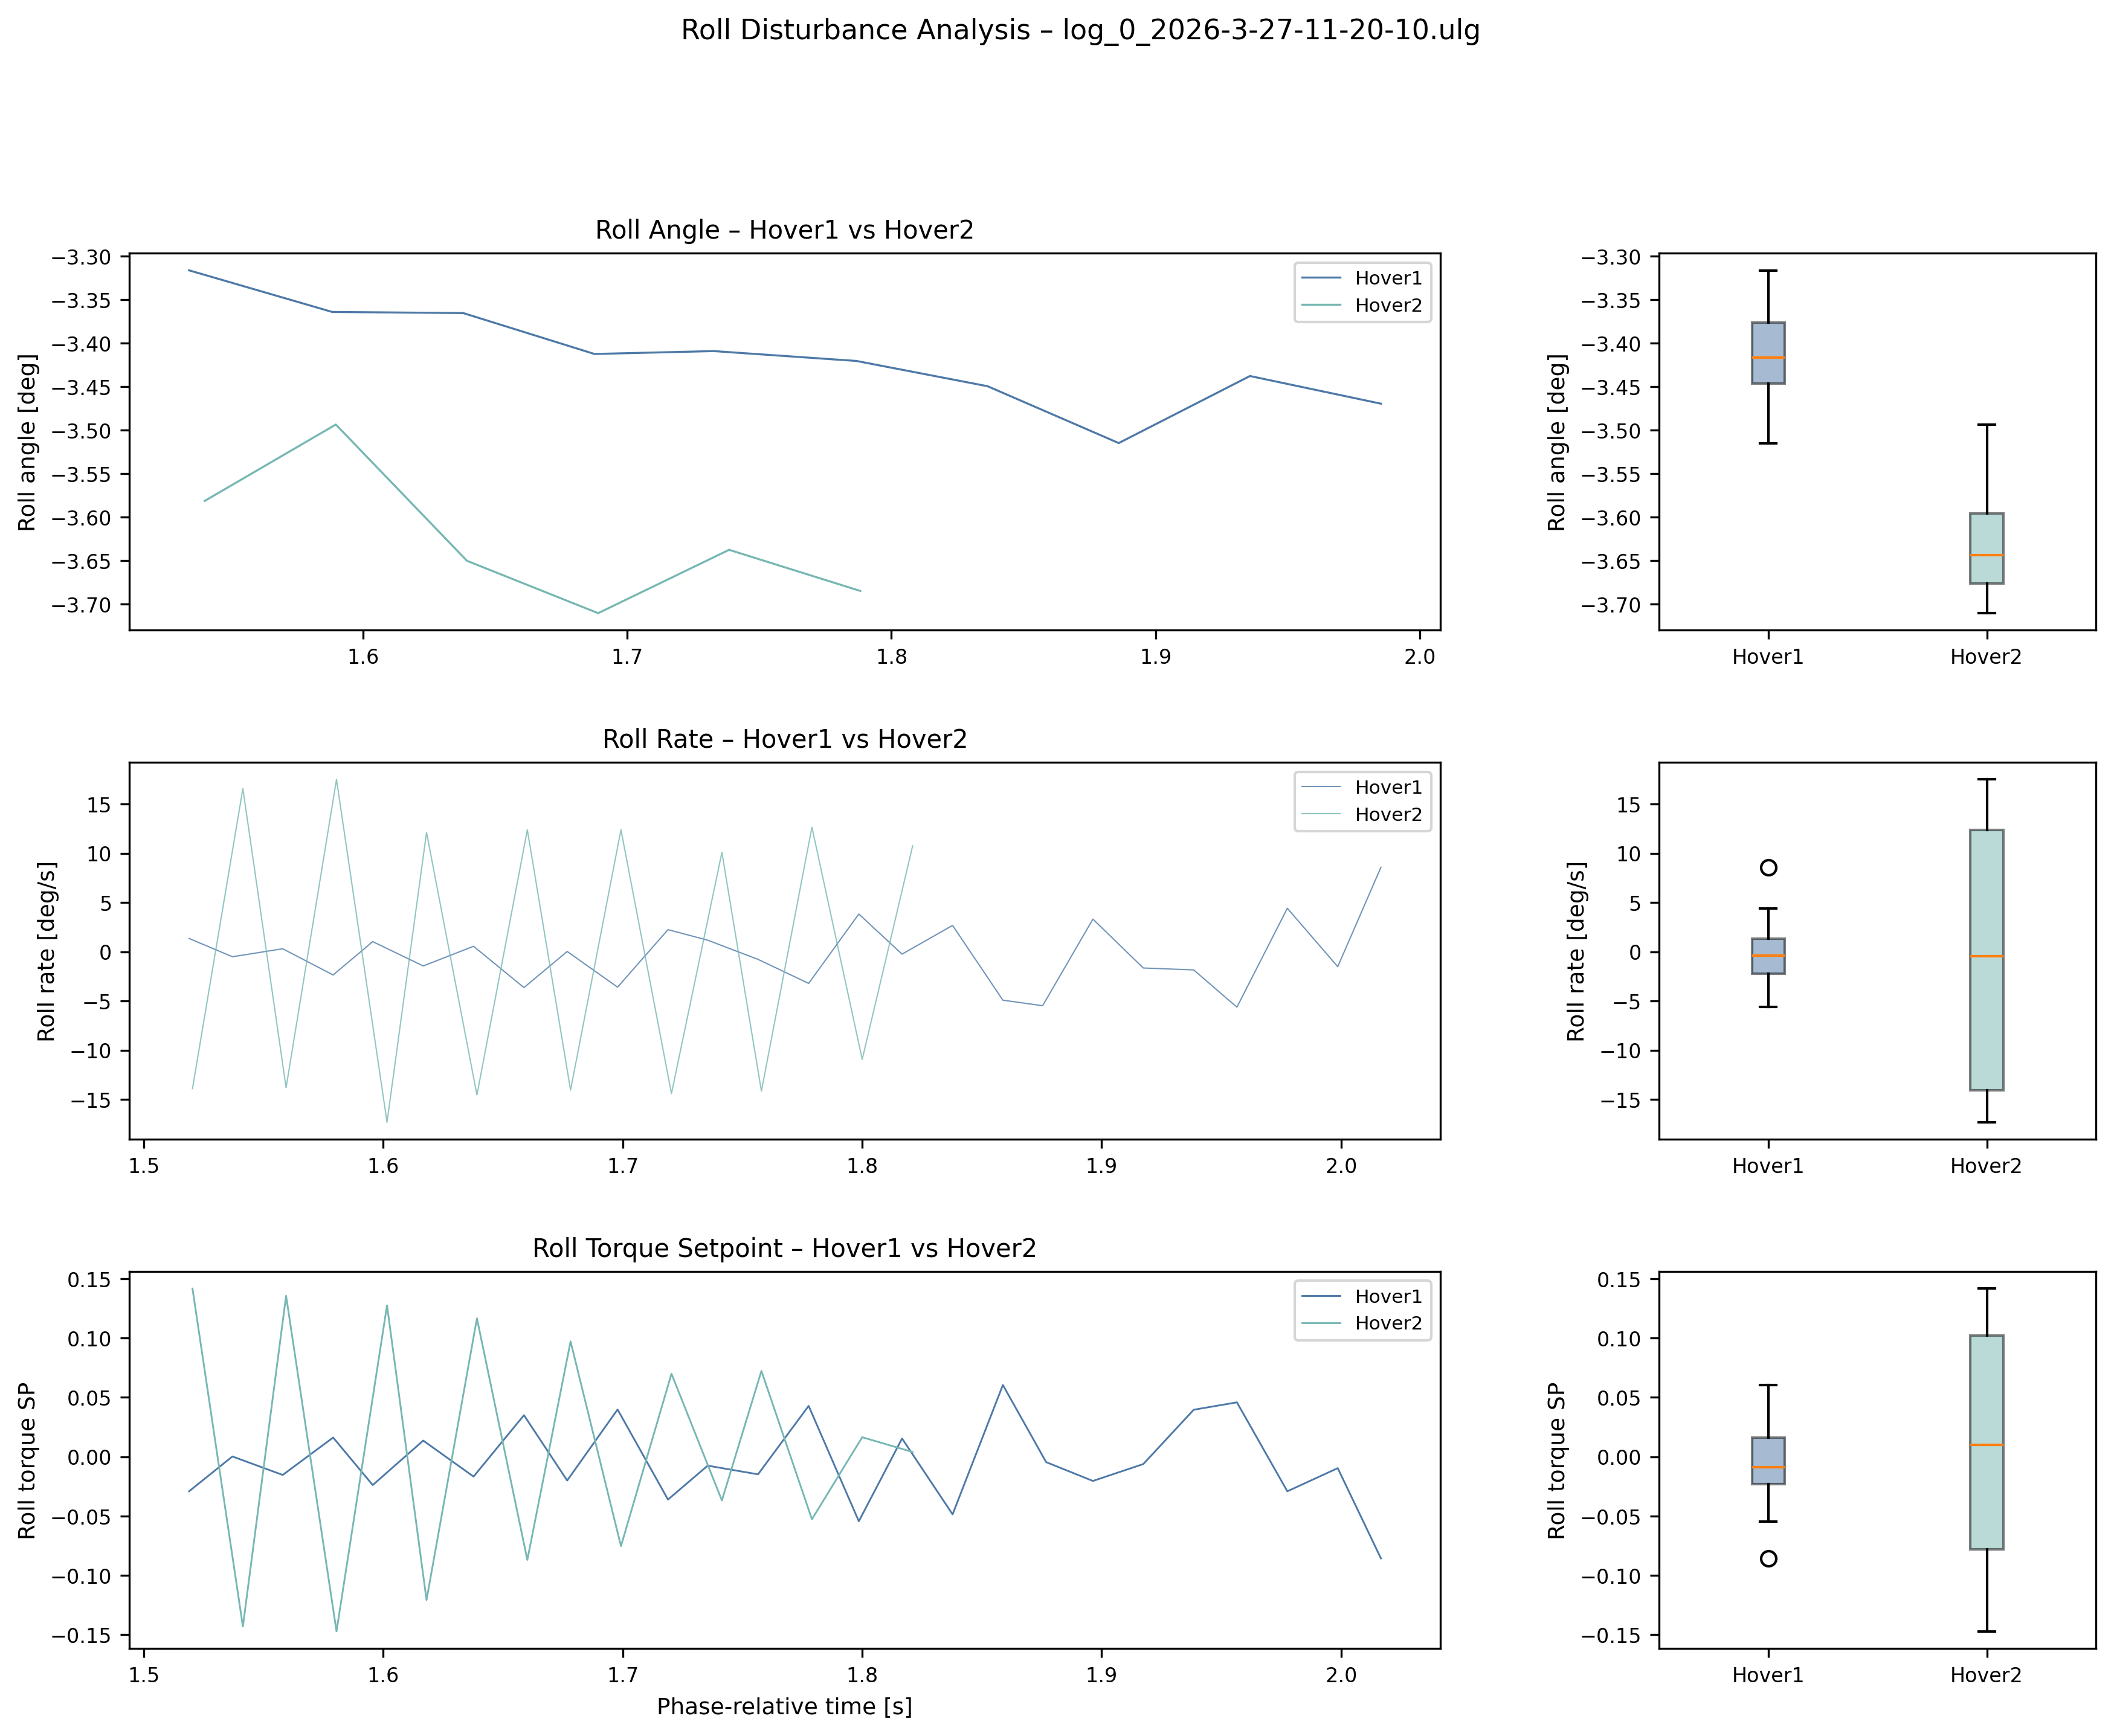
\includegraphics[width=\linewidth]{group_a/plot2_roll_detail.png}
\caption{Roll disturbance comparison between Hover1 and Hover2 for Group~A representative run. The initial 1.5\,s transient is excluded.}
\label{fig:roll_detail_a}
\end{figure}

%%%%%%%%%%%%%%%%%%%%%%%%%%%%%%%%%%%%%%%%%%%%%%%%%%%%%%%%%%%%
\section{複数ラン統計}\label{sec:multi_run}
%%%%%%%%%%%%%%%%%%%%%%%%%%%%%%%%%%%%%%%%%%%%%%%%%%%%%%%%%%%%

本章以降のすべての統計量は, ホバリングフェーズ先頭 1.5\,s を除去した安定区間のデータに基づく.

\subsection{Group B (11 ラン)}

Fig.~\ref{fig:stats_b} に Group B 全 11 ランのフェーズ別統計を示す.

\begin{figure}[H]
\centering
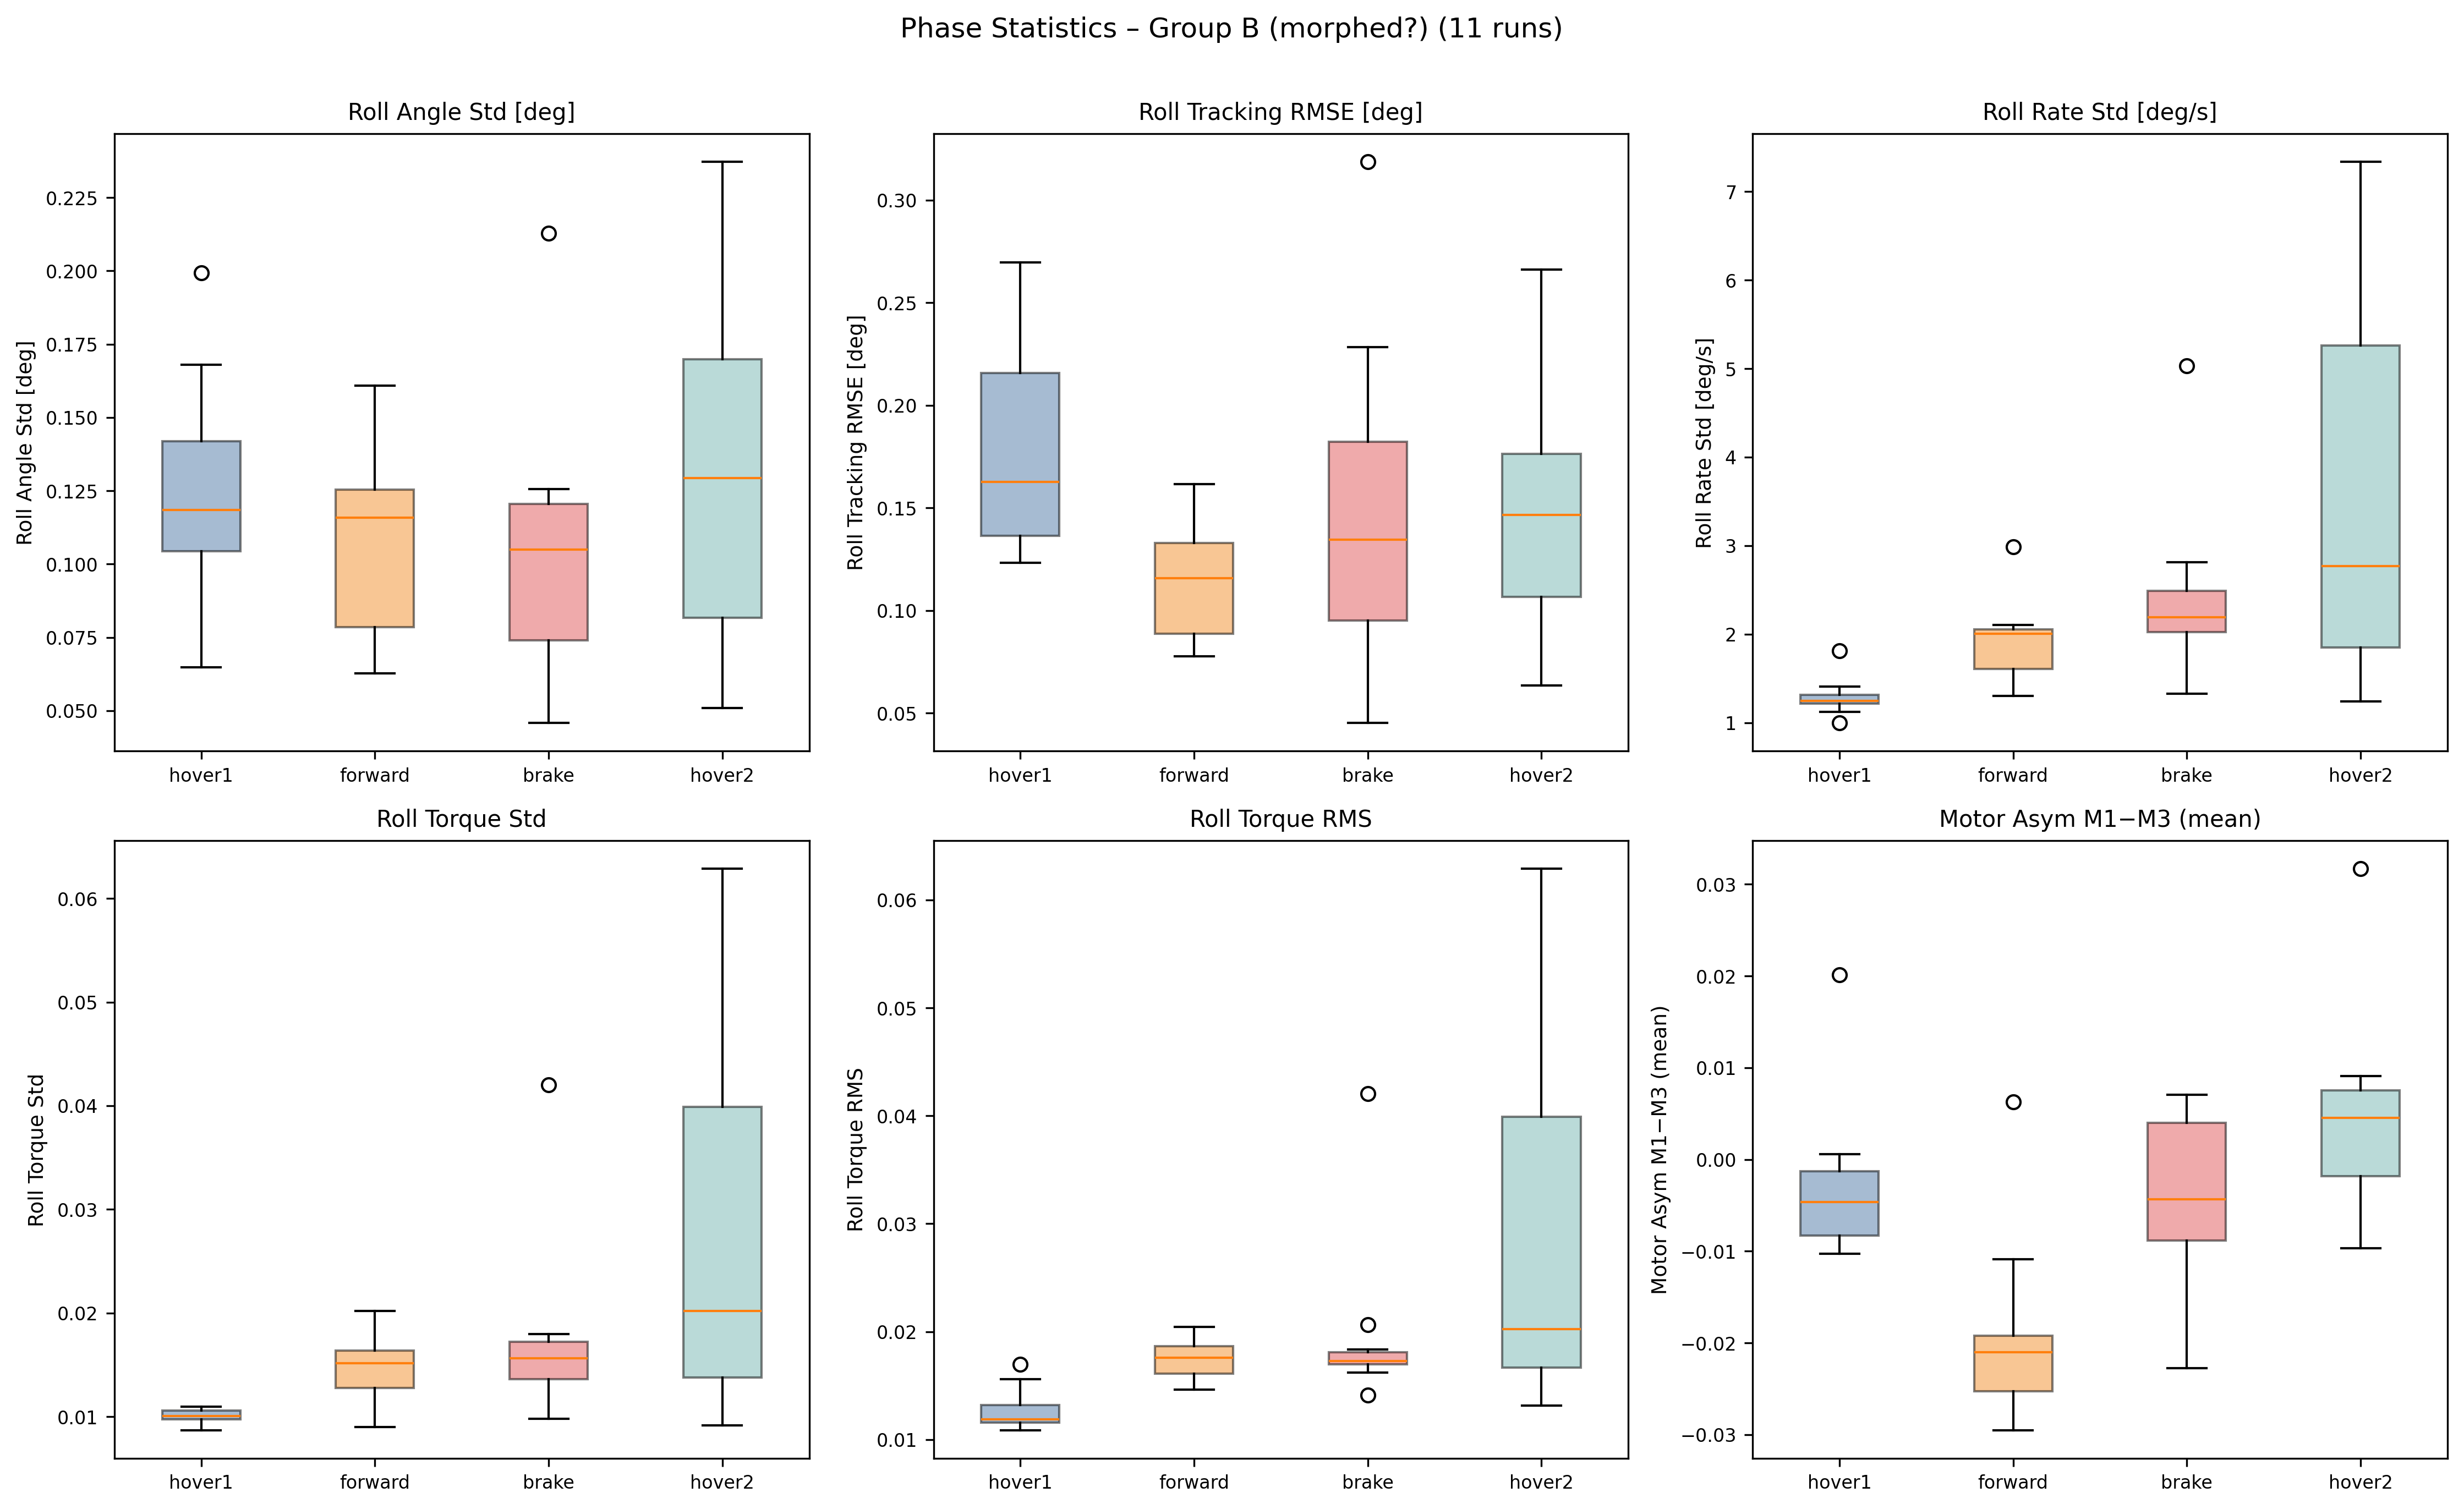
\includegraphics[width=\linewidth]{plot5_statistics_group_b.png}
\caption{Phase-wise statistics for Group~B (11 runs). Six metrics are shown as box plots across the four flight phases. Hover phases use data after 1.5\,s transient trimming.}
\label{fig:stats_b}
\end{figure}

Table~\ref{tab:paired_b} に Hover1 vs Hover2 の対応あり Wilcoxon 符号順位検定の結果を示す.

\begin{table}[H]
\centering
\caption{Paired Wilcoxon signed-rank tests: Hover1 vs.\ Hover2 for Group~B (11 runs). Hover data trimmed by 1.5\,s. Significant results ($p < 0.05$) are shown in bold.}
\label{tab:paired_b}
\begin{tabular}{lrrrrr}
\toprule
Metric & Hover1 & Hover2 & $\Delta$ & Cohen's $d$ & $p$ \\
\midrule
Roll Angle Std [deg]     & 0.126 & 0.134 & $+0.008$ & $+0.15$ & 0.520 \\
Roll Track RMSE [deg]    & 0.180 & 0.150 & $-0.030$ & $-0.53$ & 0.365 \\
Roll Rate Std [deg/s]    & 1.287 & 3.684 & $+2.398$ & $+1.54$ & \textbf{0.003} \\
Roll Torque Std          & 0.010 & 0.029 & $+0.019$ & $+1.37$ & \textbf{0.002} \\
Roll Torque RMS          & 0.013 & 0.031 & $+0.018$ & $+1.41$ & \textbf{0.007} \\
Motor Asym M1--M3        & $-0.003$ & $+0.005$ & $+0.008$ & $+0.82$ & \textbf{0.007} \\
Roll Integ Mean          & $-0.005$ & $-0.003$ & $+0.002$ & $+0.37$ & \textbf{0.042} \\
\bottomrule
\end{tabular}
\end{table}

過渡状態の除去により, Hover1 の Roll Angle Std が 0.882\,deg から 0.126\,deg に低下し, 安定状態のみが評価対象となった. その結果, 壁効果のシグナルがより明確になった:
\begin{itemize}
    \item \textbf{Roll Rate Std}: 壁近接で 2.9 倍に増大 ($d = 1.54$, $p = 0.003$)
    \item \textbf{Roll Torque Std}: 壁近接で 2.9 倍に増大 ($d = 1.37$, $p = 0.002$)
    \item \textbf{Motor Asym M1--M3}: 負から正に反転 ($d = 0.82$, $p = 0.007$)
    \item \textbf{Roll Integ Mean}: 壁近接で積分項が有意にシフト ($p = 0.042$)
\end{itemize}
トリミング前は非有意であった Roll Rate Std, Roll Torque Std が, 過渡除去後に高度に有意（$p < 0.01$）となった.

\subsection{Group A (4 ラン)}

Fig.~\ref{fig:stats_a} に Group A の統計を, Table~\ref{tab:paired_a} に検定結果を示す.

\begin{figure}[H]
\centering
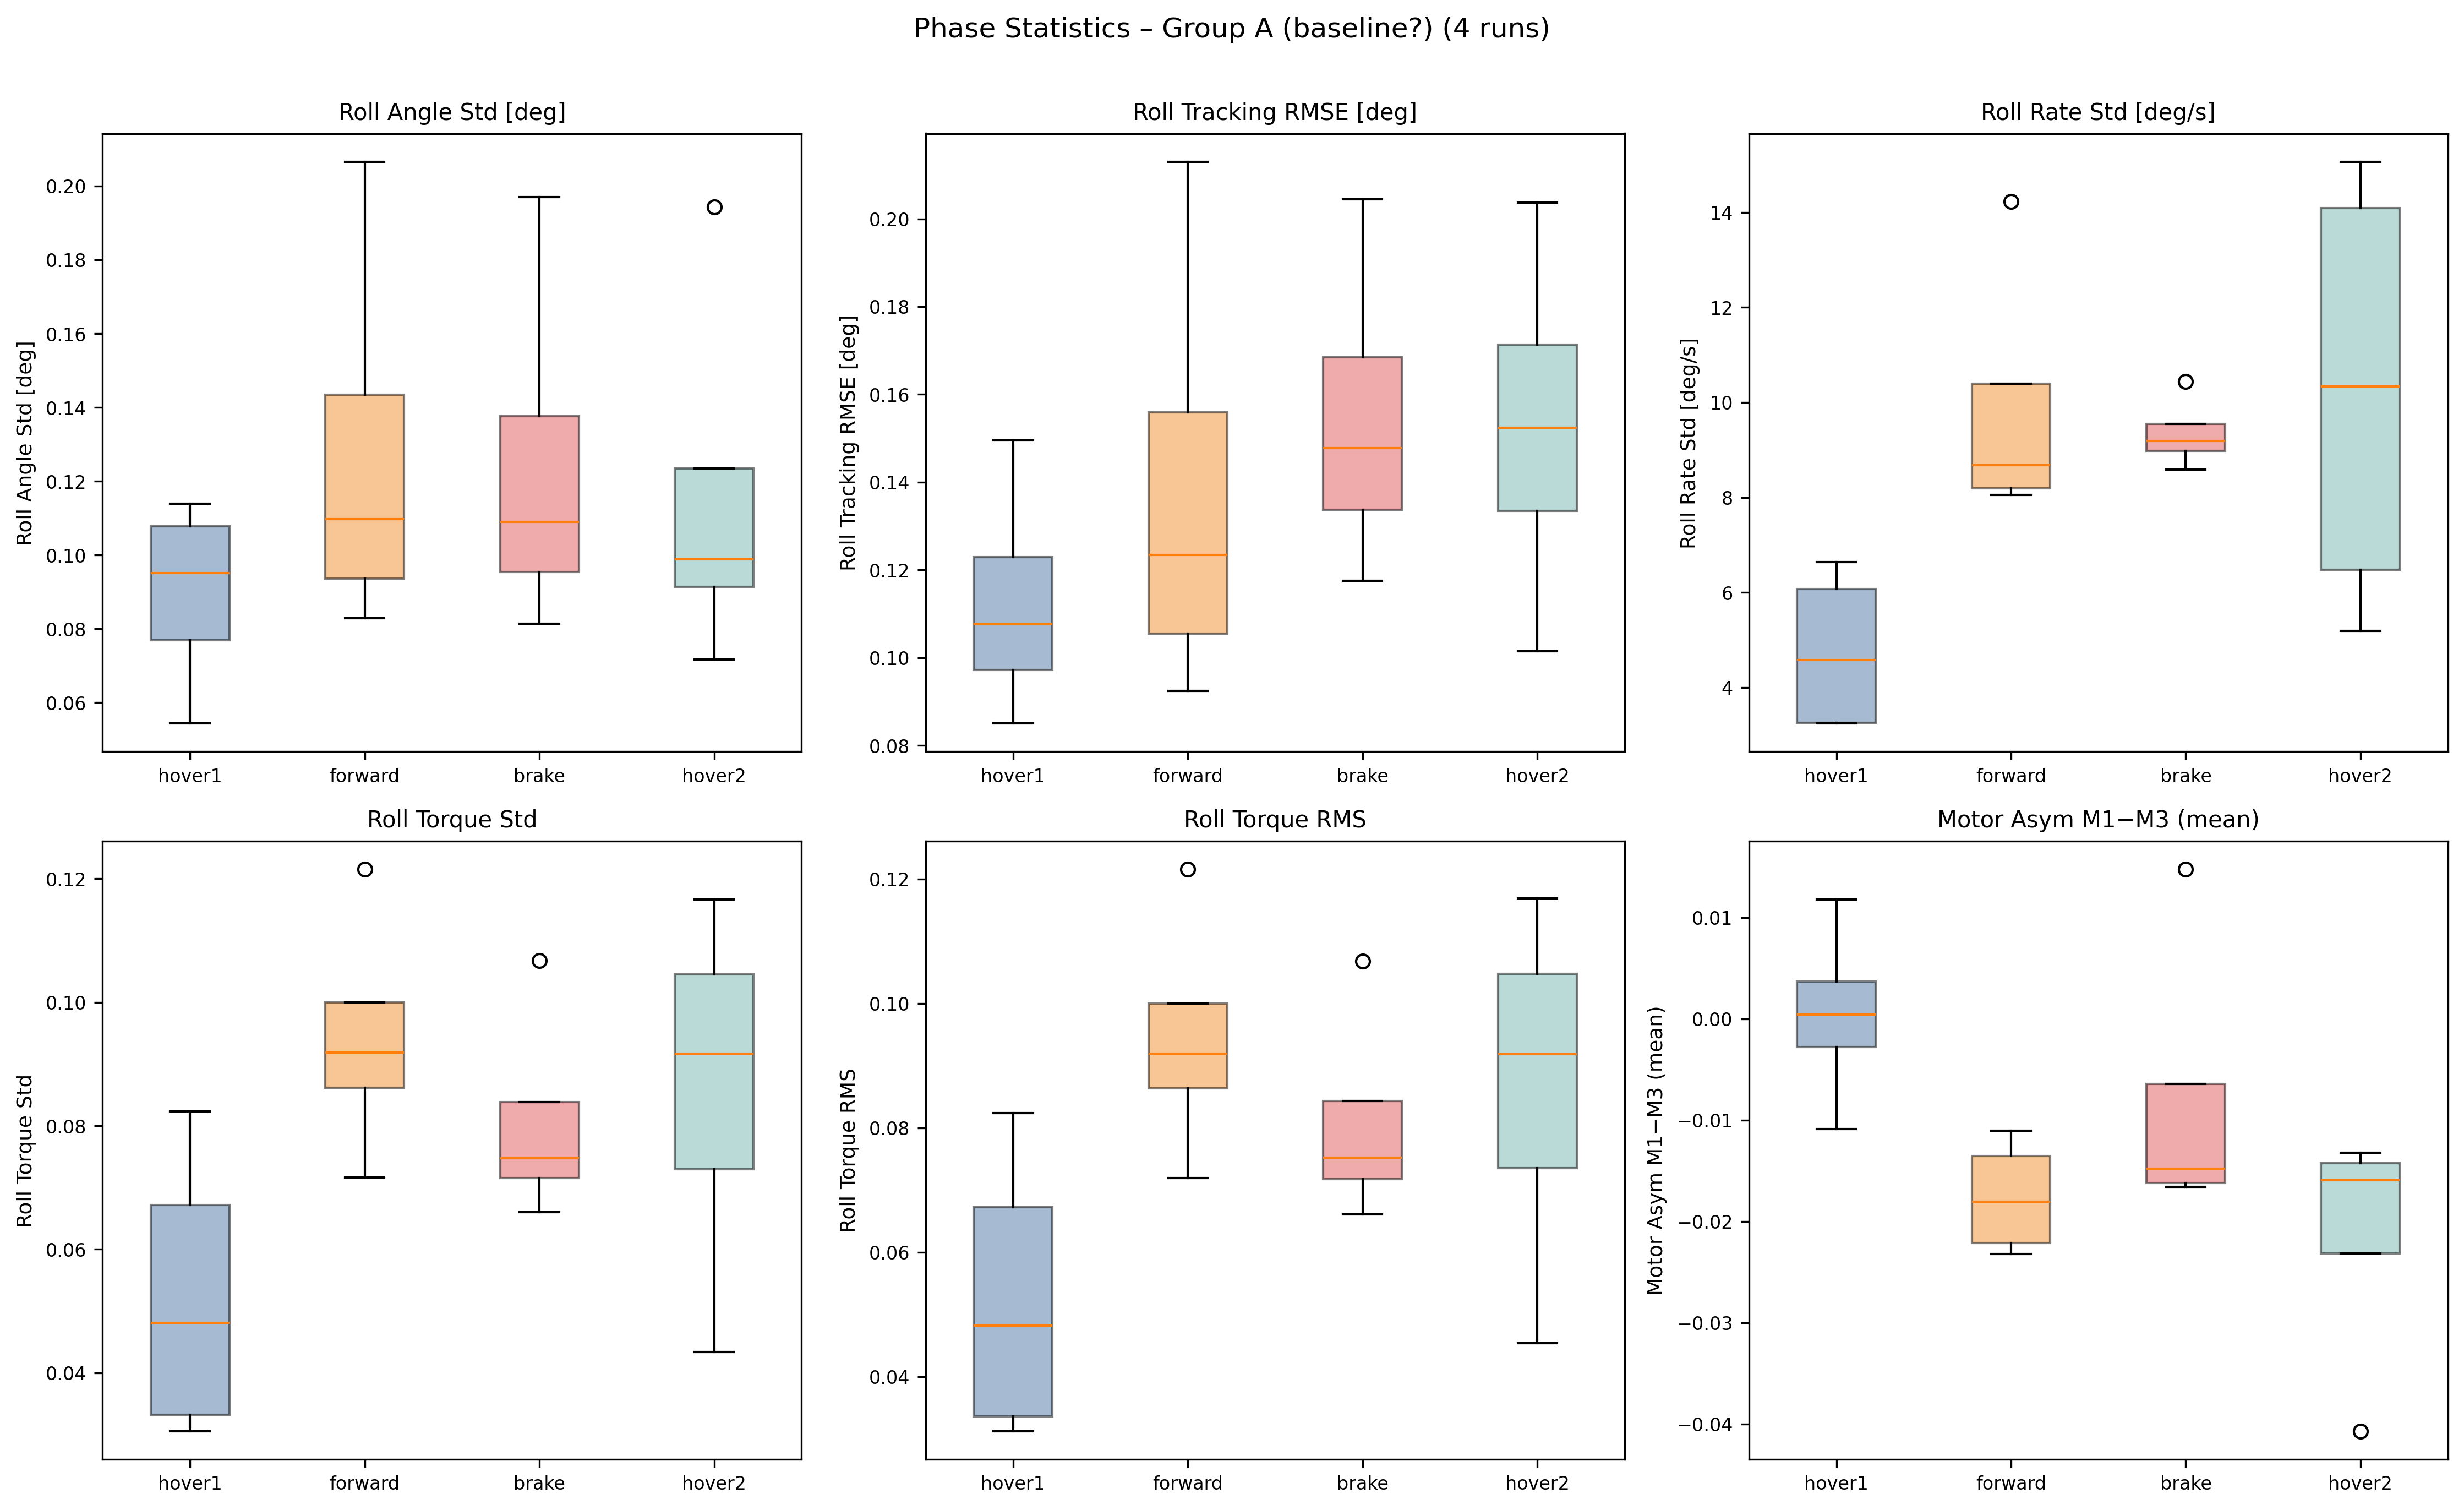
\includegraphics[width=\linewidth]{plot5_statistics_group_a.png}
\caption{Phase-wise statistics for Group~A (4 runs). Hover data trimmed by 1.5\,s.}
\label{fig:stats_a}
\end{figure}

\begin{table}[H]
\centering
\caption{Paired Wilcoxon signed-rank tests: Hover1 vs.\ Hover2 for Group~A (4 runs). Hover data trimmed by 1.5\,s. Due to the small sample size ($n=4$), the minimum achievable $p$-value is 0.125.}
\label{tab:paired_a}
\begin{tabular}{lrrrrr}
\toprule
Metric & Hover1 & Hover2 & $\Delta$ & Cohen's $d$ & $p$ \\
\midrule
Roll Angle Std [deg]     & 0.090 & 0.116 & $+0.026$ & $+0.62$ & 0.250 \\
Roll Track RMSE [deg]    & 0.112 & 0.152 & $+0.040$ & $+1.12$ & 0.125 \\
Roll Rate Std [deg/s]    & 4.756 & 10.232 & $+5.476$ & $+1.49$ & 0.125 \\
Roll Torque Std          & 0.052 & 0.086 & $+0.034$ & $+1.19$ & 0.125 \\
Roll Torque RMS          & 0.053 & 0.086 & $+0.034$ & $+1.23$ & 0.125 \\
Motor Asym M1--M3        & $+0.000$ & $-0.021$ & $-0.022$ & $-1.95$ & 0.125 \\
Roll Integ Mean          & $-0.002$ & $-0.006$ & $-0.004$ & $-1.27$ & 0.125 \\
\bottomrule
\end{tabular}
\end{table}

Group A では, 壁近接により Roll Rate Std が Hover1 の 2.2 倍に増大 ($d = 1.49$) し, Roll Torque の増大も顕著である ($d > 1.1$). 注目すべきは Motor Asym の挙動で, Group B とは逆方向（$\Delta = -0.022$, $d = -1.95$）に変化しており, 壁効果に対するモータ補償の方向が機体構成によって異なることを示唆する. ただし, サンプル数 $n = 4$ のため Wilcoxon 検定の最小 $p$ 値が 0.125 であり, 統計的有意性の判定には限界がある.

%%%%%%%%%%%%%%%%%%%%%%%%%%%%%%%%%%%%%%%%%%%%%%%%%%%%%%%%%%%%
\section{グループ間比較}\label{sec:cross_group}
%%%%%%%%%%%%%%%%%%%%%%%%%%%%%%%%%%%%%%%%%%%%%%%%%%%%%%%%%%%%

Fig.~\ref{fig:group_comparison} に, 両グループの Hover1 / Hover2 を並列比較したボックスプロットを示す.

\begin{figure}[H]
\centering
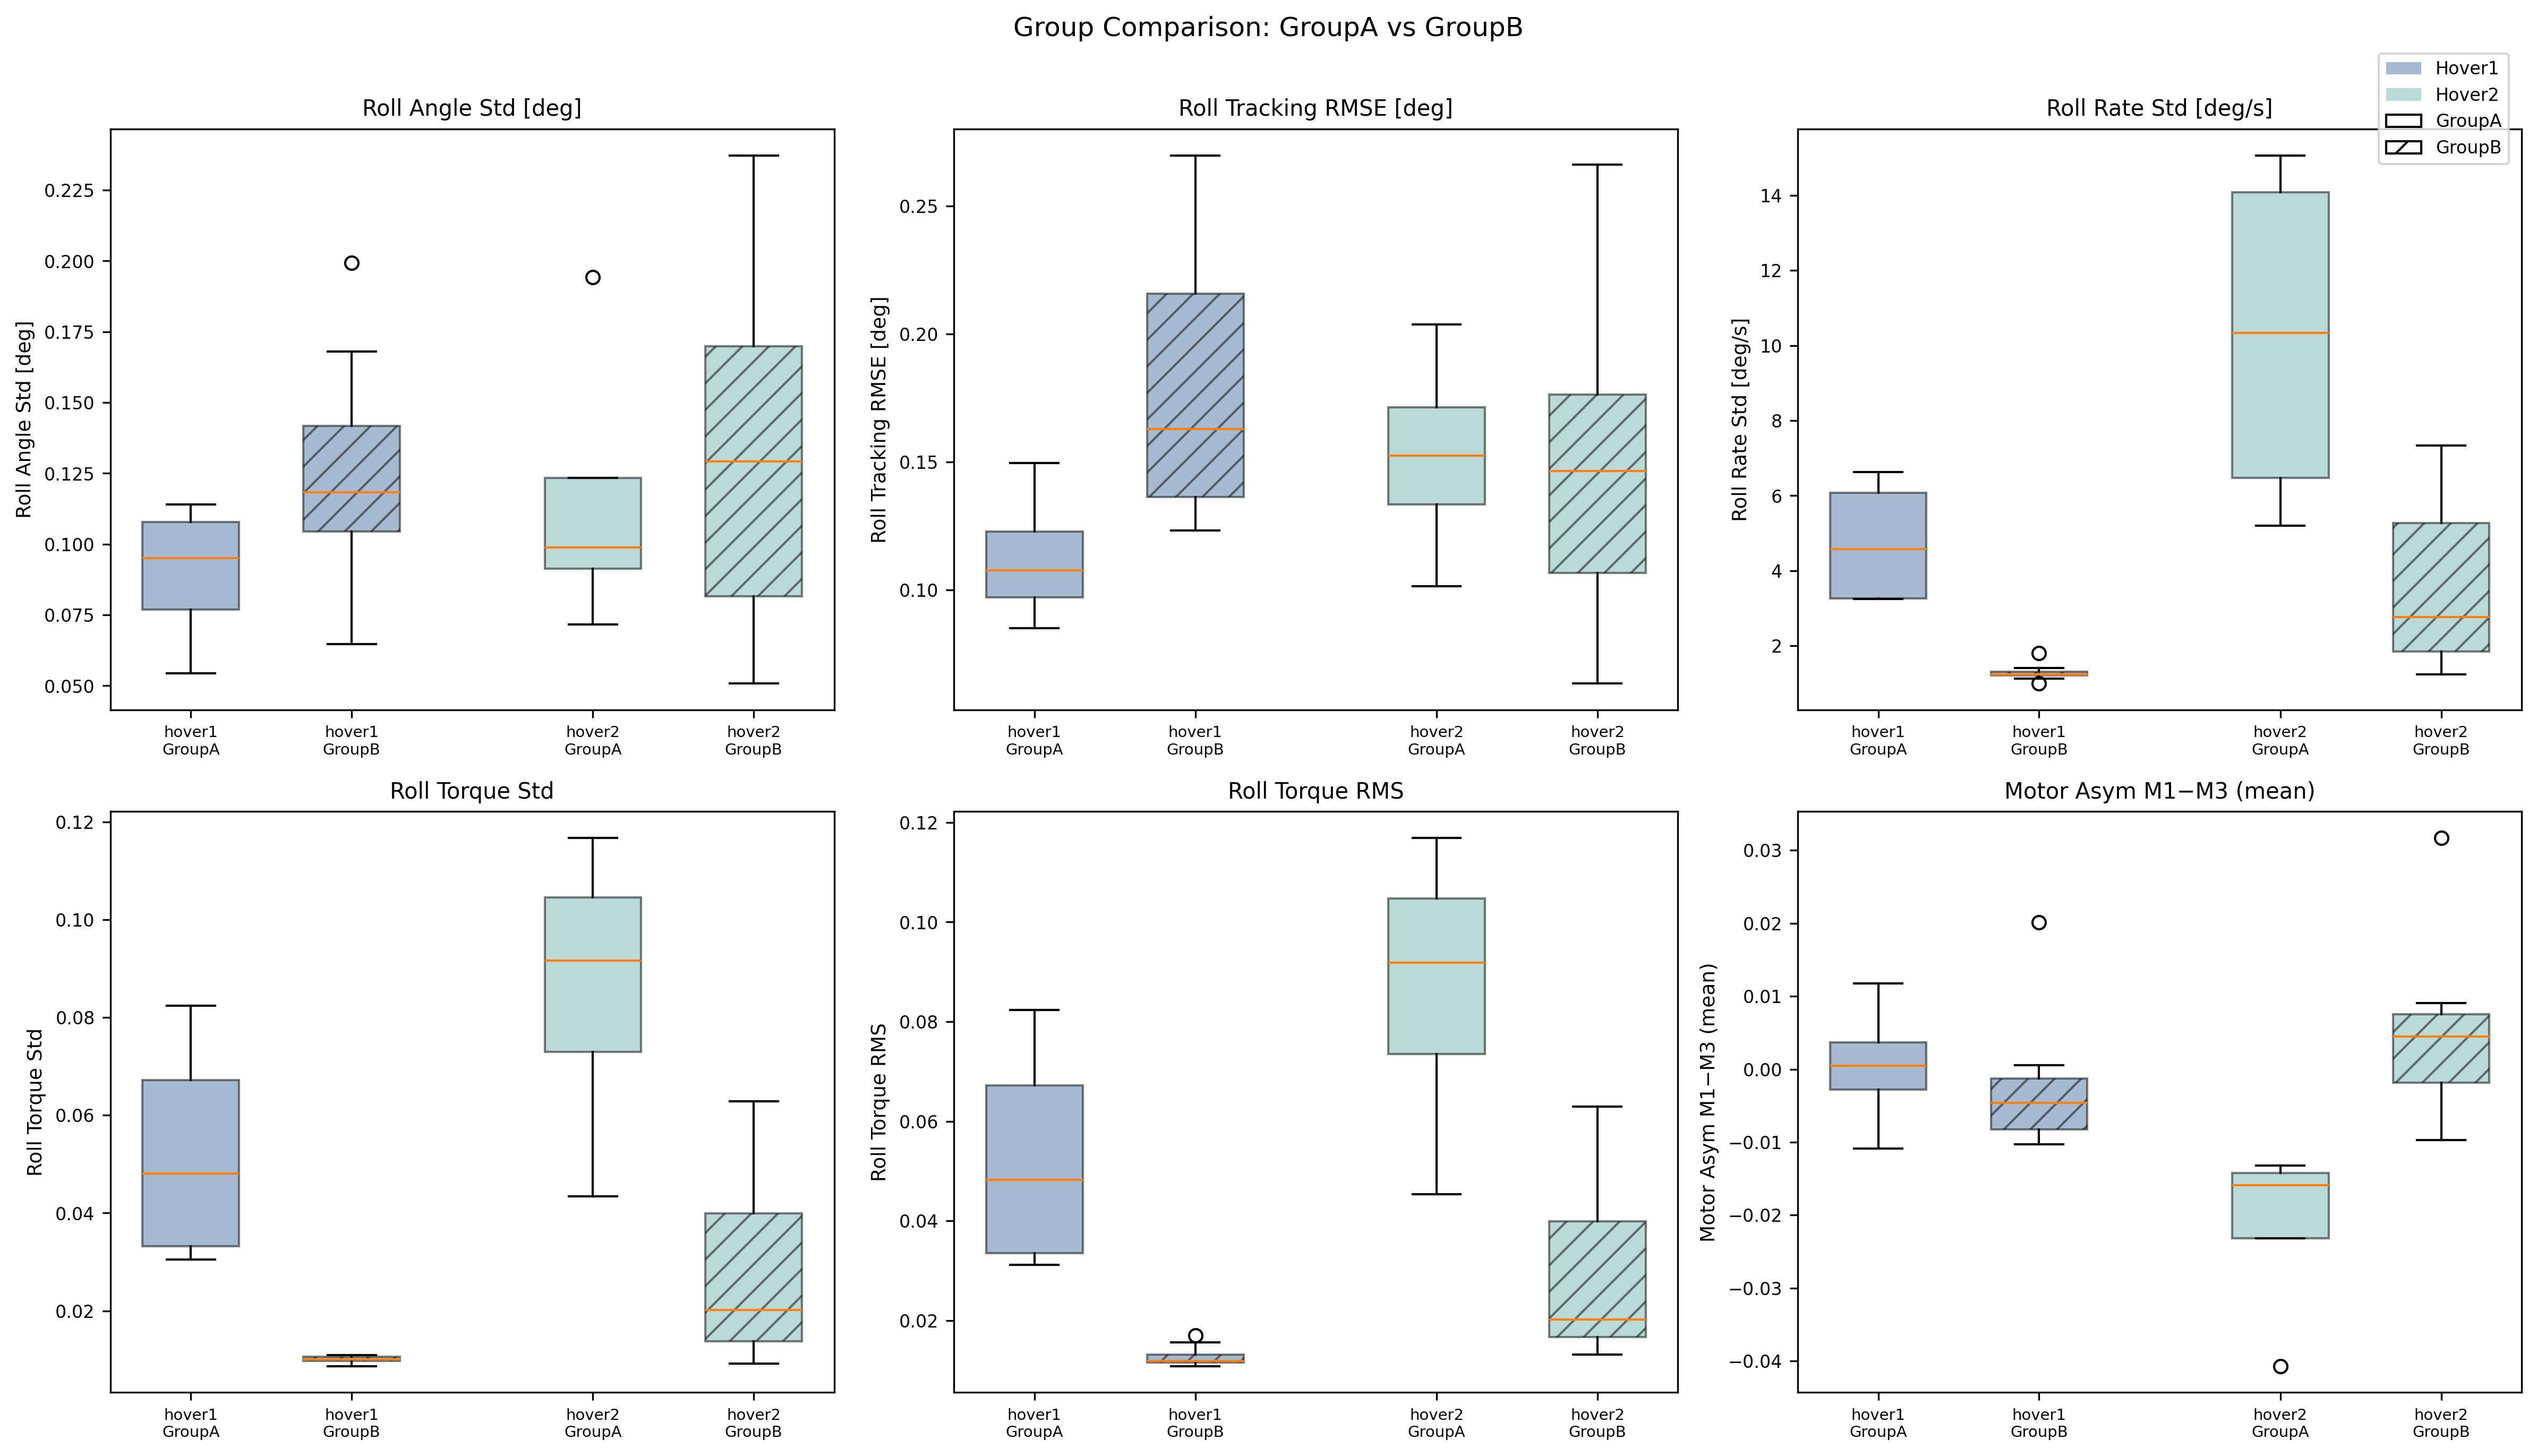
\includegraphics[width=\linewidth]{plot7_group_comparison.png}
\caption{Cross-group comparison of Hover1 and Hover2 statistics. Solid boxes: Group~A, hatched boxes: Group~B. Blue: Hover1, teal: Hover2. Hover data trimmed by 1.5\,s.}
\label{fig:group_comparison}
\end{figure}

Table~\ref{tab:cross_hover2} に Hover2 同士のグループ間比較（Mann--Whitney $U$ 検定）を示す.

\begin{table}[H]
\centering
\caption{Cross-group Mann--Whitney $U$ tests for the Hover2 phase. Significant results ($p < 0.05$) are shown in bold.}
\label{tab:cross_hover2}
\begin{tabular}{lrrrrr}
\toprule
Metric & Group~A & Group~B & $\Delta$ & Cohen's $d$ & $p$ \\
\midrule
Roll Angle Std [deg]     & 0.116 & 0.134 & $+0.018$ & $+0.31$ & 0.753 \\
Roll Track RMSE [deg]    & 0.152 & 0.150 & $-0.003$ & $-0.05$ & 0.851 \\
Roll Rate Std [deg/s]    & 10.232 & 3.684 & $-6.548$ & $-1.72$ & \textbf{0.018} \\
Roll Torque Std          & 0.086 & 0.029 & $-0.057$ & $-2.17$ & \textbf{0.006} \\
Roll Torque RMS          & 0.086 & 0.031 & $-0.056$ & $-2.22$ & \textbf{0.006} \\
Motor Asym M1--M3        & $-0.021$ & $+0.005$ & $+0.026$ & $+2.23$ & \textbf{0.002} \\
Roll Integ Mean          & $-0.006$ & $-0.003$ & $+0.003$ & $+0.54$ & 0.571 \\
\bottomrule
\end{tabular}
\end{table}

壁近接状態（Hover2）において, Group A は Group B に対して Roll Rate Std が約 2.8 倍, Roll Torque Std/RMS が約 2.8 倍大きく, いずれも高度に有意である ($p < 0.02$). さらに, Motor Asym の符号が Group A では負, Group B では正であり, 壁効果に対するモータ補償の方向自体が機体構成によって反転している ($p = 0.002$, $d = 2.23$).

ただし, この差にはコマンド条件の違い（Roll cmd: $-0.10$ vs $-0.20$）が寄与している可能性がある. トリムバイアスの影響を除去するため, 次節で Difference-in-Differences 分析を行う.

%%%%%%%%%%%%%%%%%%%%%%%%%%%%%%%%%%%%%%%%%%%%%%%%%%%%%%%%%%%%
\section{Difference-in-Differences 分析}\label{sec:did}
%%%%%%%%%%%%%%%%%%%%%%%%%%%%%%%%%%%%%%%%%%%%%%%%%%%%%%%%%%%%

各ランについて壁効果の大きさを $\Delta_i = \text{metric}(\text{Hover2}) - \text{metric}(\text{Hover1})$ として定義する. この差分をとることでトリムバイアスがキャンセルされ, 壁効果そのものの大きさをグループ間で公平に比較できる.

Fig.~\ref{fig:did} に DiD 分析結果を, Table~\ref{tab:did} に統計検定結果を示す.

\begin{figure}[H]
\centering
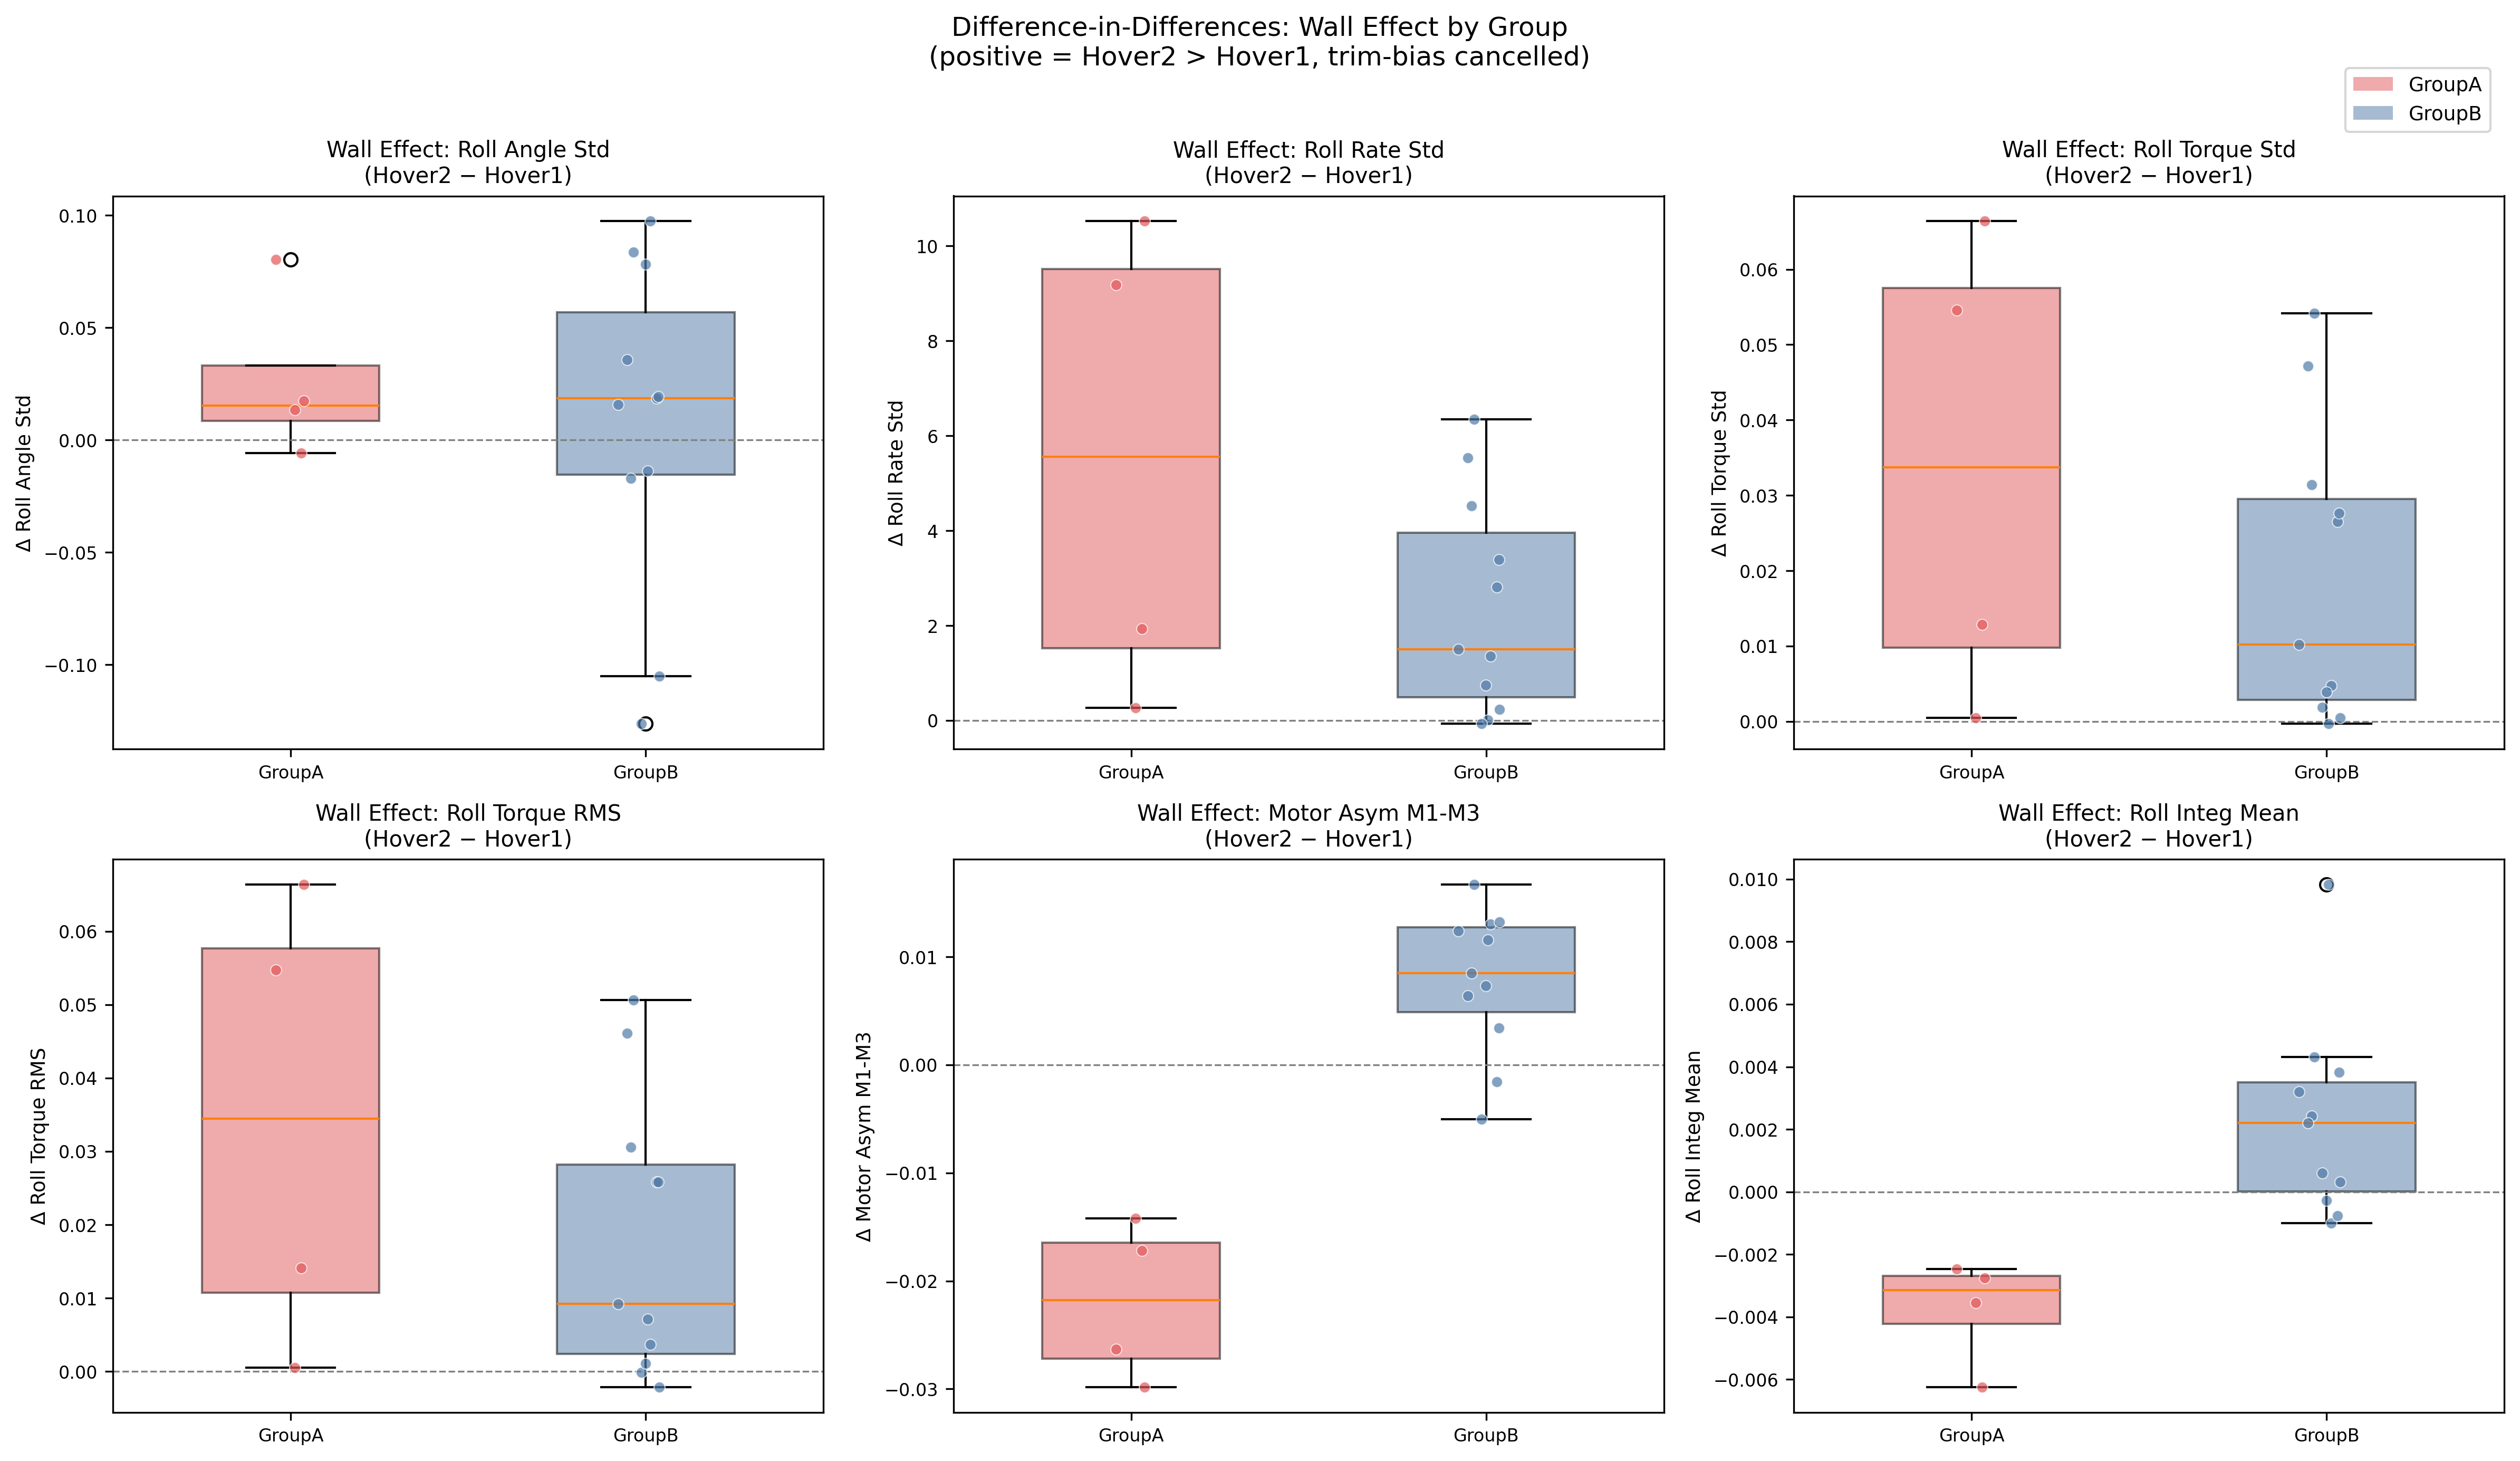
\includegraphics[width=\linewidth]{plot8_did_analysis.png}
\caption{Difference-in-Differences (DiD) analysis. Each box shows the distribution of $\Delta = \text{Hover2} - \text{Hover1}$ for the given metric, with individual data points overlaid. Positive values indicate an increase near the wall. The dashed line marks zero (no wall effect). Hover data trimmed by 1.5\,s.}
\label{fig:did}
\end{figure}

\begin{table}[H]
\centering
\caption{Difference-in-Differences: wall-effect magnitude ($\Delta = \text{Hover2} - \text{Hover1}$) by group. Mann--Whitney $U$ test. Significant results ($p < 0.05$) are shown in bold.}
\label{tab:did}
\begin{tabular}{lrrrrr}
\toprule
Metric & Group~A $\Delta$ & Group~B $\Delta$ & DiD diff & Cohen's $d$ & $p$ \\
\midrule
Roll Angle Std      & $+0.026$ & $+0.008$ & $-0.019$ & $-0.32$ & 1.000 \\
Roll Rate Std       & $+5.476$ & $+2.398$ & $-3.079$ & $-0.78$ & 0.280 \\
Roll Torque Std     & $+0.034$ & $+0.019$ & $-0.015$ & $-0.56$ & 0.343 \\
Roll Torque RMS     & $+0.034$ & $+0.018$ & $-0.016$ & $-0.61$ & 0.343 \\
Motor Asym M1--M3   & $-0.022$ & $+0.008$ & $+0.030$ & $+4.21$ & \textbf{0.002} \\
Roll Integ Mean     & $-0.004$ & $+0.002$ & $+0.006$ & $+2.38$ & \textbf{0.002} \\
\bottomrule
\end{tabular}
\end{table}

\subsection{解釈}

過渡状態を除去した DiD 分析から, 以下の知見が得られた:

\begin{enumerate}
    \item \textbf{モータ非対称度の壁効果が機体構成で反転} ($d = 4.21$, $p = 0.002$).
    Group A では壁近接により M1--M3 非対称が負方向に変化（$\Delta = -0.022$）するのに対し, Group B では正方向に変化（$\Delta = +0.008$）する. これは壁効果に対するモータ補償の方向が機体変形により逆転していることを意味し, 極めて大きな効果量（Cohen's $d = 4.21$）を示す.

    \item \textbf{レート制御積分項の壁効果も反転} ($d = 2.38$, $p = 0.002$).
    Group A では壁近接で Roll 積分項が負方向に蓄積（定常外乱の補償）するのに対し, Group B では正方向に微増しており, 定常外乱の性質が機体構成で異なることを示す.

    \item \textbf{Roll Rate / Torque の壁効果の大きさ}は, Group A が Group B の 1.8〜2.3 倍であり中〜大効果量（$d = 0.56$--$0.78$）を示すが, Group A の $n = 4$ のため統計的有意水準には到達していない.
\end{enumerate}

%%%%%%%%%%%%%%%%%%%%%%%%%%%%%%%%%%%%%%%%%%%%%%%%%%%%%%%%%%%%
\section{考察}\label{sec:discussion}
%%%%%%%%%%%%%%%%%%%%%%%%%%%%%%%%%%%%%%%%%%%%%%%%%%%%%%%%%%%%

\subsection{主要な発見}

\begin{enumerate}
    \item \textbf{壁効果の存在}: 両グループともに, 壁近接時（Hover2）で Roll 方向の外乱指標（角速度変動, トルク指令変動, モータ非対称性）が定常状態から有意に増大しており, 制御ログからも壁効果が明確に検出された. 特に Group B では Roll Rate Std ($p = 0.003$), Roll Torque Std ($p = 0.002$), Motor Asym ($p = 0.007$) のいずれも高度に有意である.

    \item \textbf{機体変形による壁効果応答の質的変化}: DiD 分析で最も顕著な発見は, モータ非対称度の壁効果の方向が機体構成により反転している点である ($d = 4.21$). これは単なる壁効果の大小ではなく, 壁効果に対する機体の空力応答が質的に異なることを意味する. ベンチ台 6 軸力センサ計測で報告されているロータ姿勢変形による壁効果モーメントの抑制・反転と定性的に整合する.

    \item \textbf{制御系からの壁効果の定量化}: 6 軸力センサなしでも, フライトログに記録される制御トルク指令・レート制御積分項・モータ出力非対称性から壁効果の大きさと方向を推定できることが示された.
\end{enumerate}

\subsection{過渡除去の効果}

ホバリングフェーズ先頭 1.5\,s のトリミングにより, 統計分析の品質が大幅に改善された. トリミング前は, アーム直後のスピンアップ過渡が Hover1 のばらつきを支配し, 壁効果のシグナルがノイズに埋もれていた. トリミング後, Group B の Hover1 Roll Angle Std は 0.882\,deg から 0.126\,deg に低下し, Roll Rate Std と Roll Torque Std が新たに有意（$p < 0.01$）となった.

\subsection{ベンチ台計測との関係}

ベンチ台計測（6 軸力センサ）では, ロータ姿勢の変形により壁効果モーメントの peak-to-peak 振幅が最大 90\% 低減されることが報告されている. 本フライトログ解析では, 直接的なモーメント計測はないものの, 制御系が出力する Roll トルク指令の RMS が Group B で Group A の約 1/3 であり ($0.031$ vs $0.086$), 壁効果モーメントの低減と整合する. さらに, モータ非対称度の反転は, 壁効果モーメントの符号が変形により変わりうるというベンチ台計測の知見を支持している.

\subsection{限界と今後の課題}

\begin{itemize}
    \item Group A / Group B がそれぞれベースライン / 変形機体であるかの確定的な記録がなく, 本解析はデータ特性からの推定に基づいている.
    \item Group A は $n = 4$ であり, 統計的検出力に限界がある. 追加実験によるサンプル数の増加が望ましい.
    \item Group A 内で \texttt{log\_0010} のみ Roll cmd が他 3 本と異なり ($-0.16$ vs $-0.10$), 完全に同一条件のグループとは言えない.
    \item 壁面距離の時間変化が直接計測されていないため, Forward/Brake フェーズにおける壁距離と外乱の相関関係を厳密に評価できない.
    \item ホバリングトリミング時間 (1.5\,s) の選択は, 時系列の目視確認に基づいており, 感度分析を行うことで妥当性を強化できる.
\end{itemize}

\end{document}
